\documentclass[l4proj.tex]{subfiles}
\begin{document}    

This chapter discusses the design choices behind RViT including the system architecture, user interface and the rationale behind the development tools chosen. 

\section{System Architecture}

The system architecture was designed based on the three-tier architecture pattern (\cite{IBM3Tier}), comprised of a presentation tier, an application tier and a data tier as seen in \textbf{Fig. \ref{fig:achitecture pattern}}. The presentation tier is responsible for communicating with the end user via the user interface. The application, or logic, tier is responsible for the core functionality of RViT as it processes the information passed from the presentation tier and augments the data layer. Finally, the data tier manages and stores the information processed by the application tier.

\begin{figure}[h!]
\begin{center}
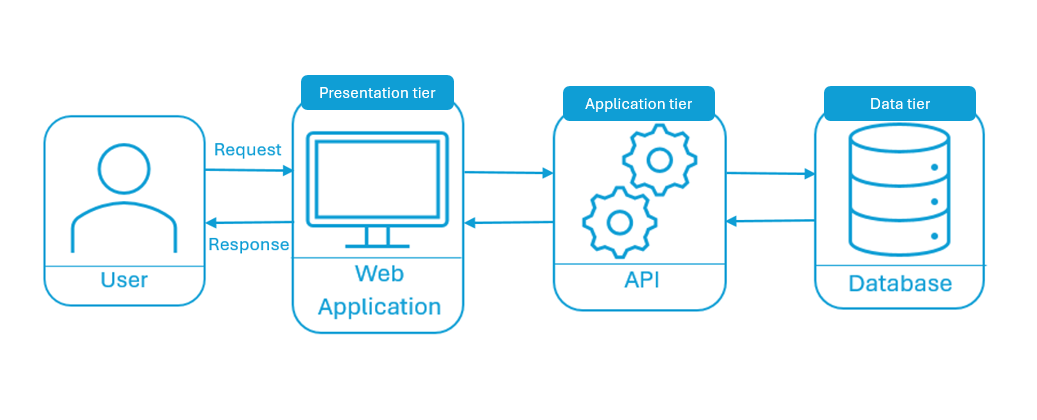
\includegraphics[scale=0.6]{dissertation/images/System Architecture.png}
\caption{System architecture diagram}
\label{fig:achitecture pattern} 
\end{center}
\end{figure}

The main advantage of the three-tier architecture design is the modularisation that it provides. Having a modular architecture leads to clear separation of concerns, meaning that each tier can be tested and developed separately. The inclusion of the application tier between the presentation and data tiers also can increase the security of the application. As there is no direct communication between the presentation and data tiers, common vulnerabilities such as SQL injections can be easily mitigated (\cite{IBM3Tier}).

Another advantage of modularisation cited by Martin Fowler is the reduced scope of attention (\cite{Fowler2015}). By separating the tiers, they can be focused on independently. This means that when working on one tier of the system, the others can be abstracted and mostly ignored. For example, when working on the presentation tier, it was possible to primarily focus on the user interface, with not no need to consider \textit{how} the application tier worked, only what information would be sent to the presentation tier. If further development occurs, this architecture would allow a development team to work on the three tiers concurrently, increasing throughput.

\section{API}
A REST API was chosen to become the application tier for a variety of reasons. These are the most widely used type of web API with Postman's 2023 State of the API report finding that 86\% of respondents used REST architecture in their APIs (\cite{Postman2023}). REST APIs also are more scalable and flexible than other architectures, such as SOAP (\cite{AWS}). The REST API approach also allows for the transfer of data in many different forms, including JSON and plain text whereas SOAP APIs can only receive and return XML data. REST APIs are also stateless, allowing them to scale easily, as opposed to SOAP APIs which must maintain a record of all previous states. REST APIs are also more efficient than their SOAP counterparts as they typically transport smaller, less complex messages (\cite{AWS}).

Another reason an API approach was chosen lies in its potential to foster innovation in future development. As discussed in \textbf{Section 2.2}, established project management tools such as Jira and Trello have marketplaces where independent developers can use published REST APIs to create custom plugins and third-party applications. By creating a REST API in the initial stages of the project, this simplifies the process if marketplace-type functionality was added in future development. 

Since REST APIs are independent of any client-side technologies used (\cite{PostmanBlog2023}), the API that was created for the RViT web application can be seamlessly reused in future development, for example developing a RViT mobile application, without requiring any modifications to the API. 


\subsection{API-first Approach}
When building the RViT API, an API-first approach was used. This is a design approach where APIs are treated as 'first class citizens' (\cite{Wagner(Swagger)}), meaning that before any code is written, the relevant API calls and responses are first defined. This approach helps to ensure that a good quality API is created, and fewer API-related failures occur. In Postman's 2023 State of the API report API-first development teams were found to be less likely to encounter API failures and had significantly quicker recovery times than non-API-first teams (\cite{PostmanAPIFirst}). 


\section{User Interface}
The majority of the functional requirements identified in \textbf{Section 3.2} involve user interaction with the application, therefore this user interface design was highly important. The aim of RViT is to provide a streamlined, easy-to-use agile project management tool, so an uncluttered user interface is required. To be able to compete with other, more established tooling, designing an aesthetically pleasing application was also prioritised. 

When analysing the user scenarios, it was identified that the primary use case of the tool would be on a desktop or laptop, so it was decided against also designing for mobile phone use. Thus other must have and should have requirements were prioritised instead.


\subsection{Initial prototyping}
Before beginning the implementation of each web page in the application, a prototyping phase was carried out. Multiple low fidelity wireframes were created for each page before a higher fidelity finalised wireframe was created as seen in \textbf{Fig. \ref{fig:figma designs}}. Figma was chosen to create the wireframes to allow for the reuse of components such as user stories and epics. Colour also became an important factor of the user interface design, so using a digital tool allowed for easy colour visualisation. Figma also allowed for a centralised location for all the created wireframes, which was especially helpful when creating consistent visual metaphors. The ability to easily access the set of finalised wireframes was essential, as due to the agile method of working, the majority of pages were designed asynchronously. So being able to compare newly created designs with previously created ones allowed the maintaining of a consistent page style through the application. 


\begin{figure}[h!]
\centering
\begin{subfigure}{.5\textwidth}
\centering
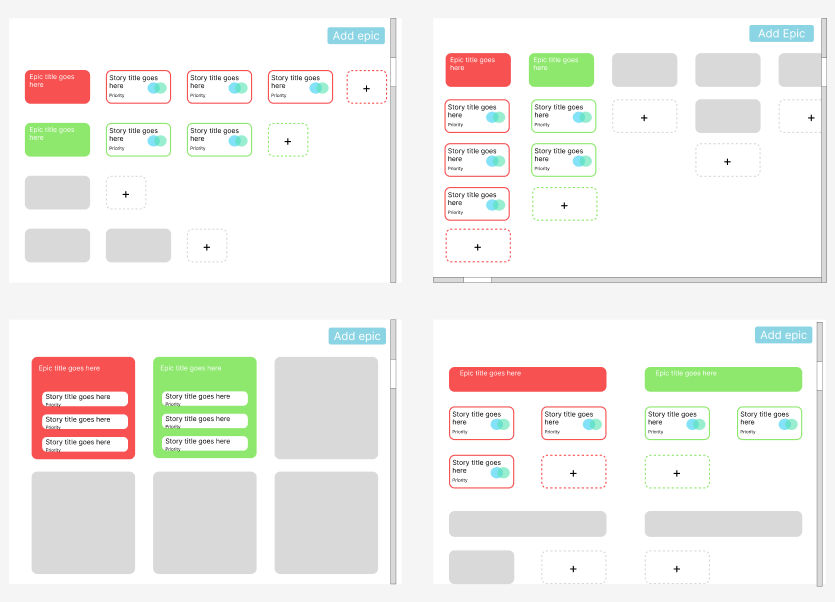
\includegraphics[scale=0.4]{dissertation/images/FigmaProtoyping.png}
\caption{Initial low fidelity wireframes for the Epics Dashboard}
\end{subfigure}%
\begin{subfigure}{.5\textwidth}
\centering
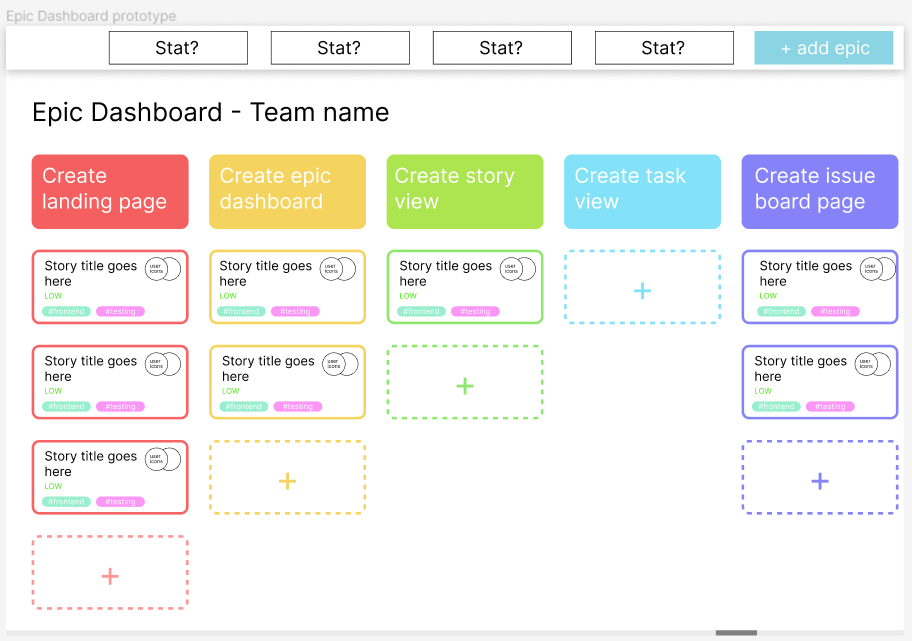
\includegraphics[scale=0.37]{dissertation/images/FinalisedEpicDashboardDesign.png}
\caption{Finalised Epics Dashboard wireframes}
\end{subfigure}

\caption{Initial vs finalised Epics Dashboard wireframes}
\label{fig:figma designs}
\end{figure}

Individual components also went through a similar prototyping phase. This was especially helpful to visualise the positioning of forms and their respective fields. 

During implementation, small interface details were changed as the user workflow was more thoroughly explored and initial feedback was obtained.



\subsection{Epics Dashboard}
A core set of RViT's must and should have functional requirements involved the ability to add, edit and prioritise epics and user stories. As these tasks were similar to each other, it was decided that these should be fulfilled by one page to reduce navigational overhead. The finalised Epic Dashboard page can be seen in \textbf{Fig. \ref{fig:epics dashboard}}.

Both team lead and team member users can access the epics dashboard of any teams they belong to. Any epics a team have defined are displayed on a horizontal line with a user-defined colour as the background and white text to satisfy \textbf{MH.5}.  User stories can be added to epics through the 'add story' button that appears below each epic. The stories associated with an epic will be displayed vertically below the epic with a border corresponding to the epic's colour, fulfilling \textbf{MH.5}. Epics can be rearranged by priority horizontally, while stories can be reordered vertically within their epic, again to visualise priority. This satisfies requirements \textbf{SH.1} and \textbf{SH.2}. This dashboard design was chosen to maximise the use of both horizontal and vertical space to allow for as much information to be displayed as possible without leading to a cluttered user interface.

It was decided to let users self-define epic colours so they could account for team members with vision impairments while still allowing for maximum customisability, fulfilling \textbf{SH.4}. A reactive element example was also included in all forms with a colour picker, so users can see instant visual feedback and ensure readability. Additionally, to ensure visibility of system status, when reordering epics and user stories, colour feedback should be displayed to the user so they can understand where elements can be moved.

Authorised users can also filter the Epics Dashboard to include all epics and user stories, only the currently incomplete epics and user stories, and only the completed epics and user stories, fulfilling requirement \textbf{CH.3}. It was identified that the majority of users would want to access only the currently incomplete epics and user stories, so this was made the default view.

As with all team-based dashboards, a team lead or team member user can switch between the dashboards of the teams they are part of by using the drop-down menu located in the top left corner of the dashboard. This fulfils requirement \textbf{MH.10}.

\begin{figure}[h!]
\begin{center}
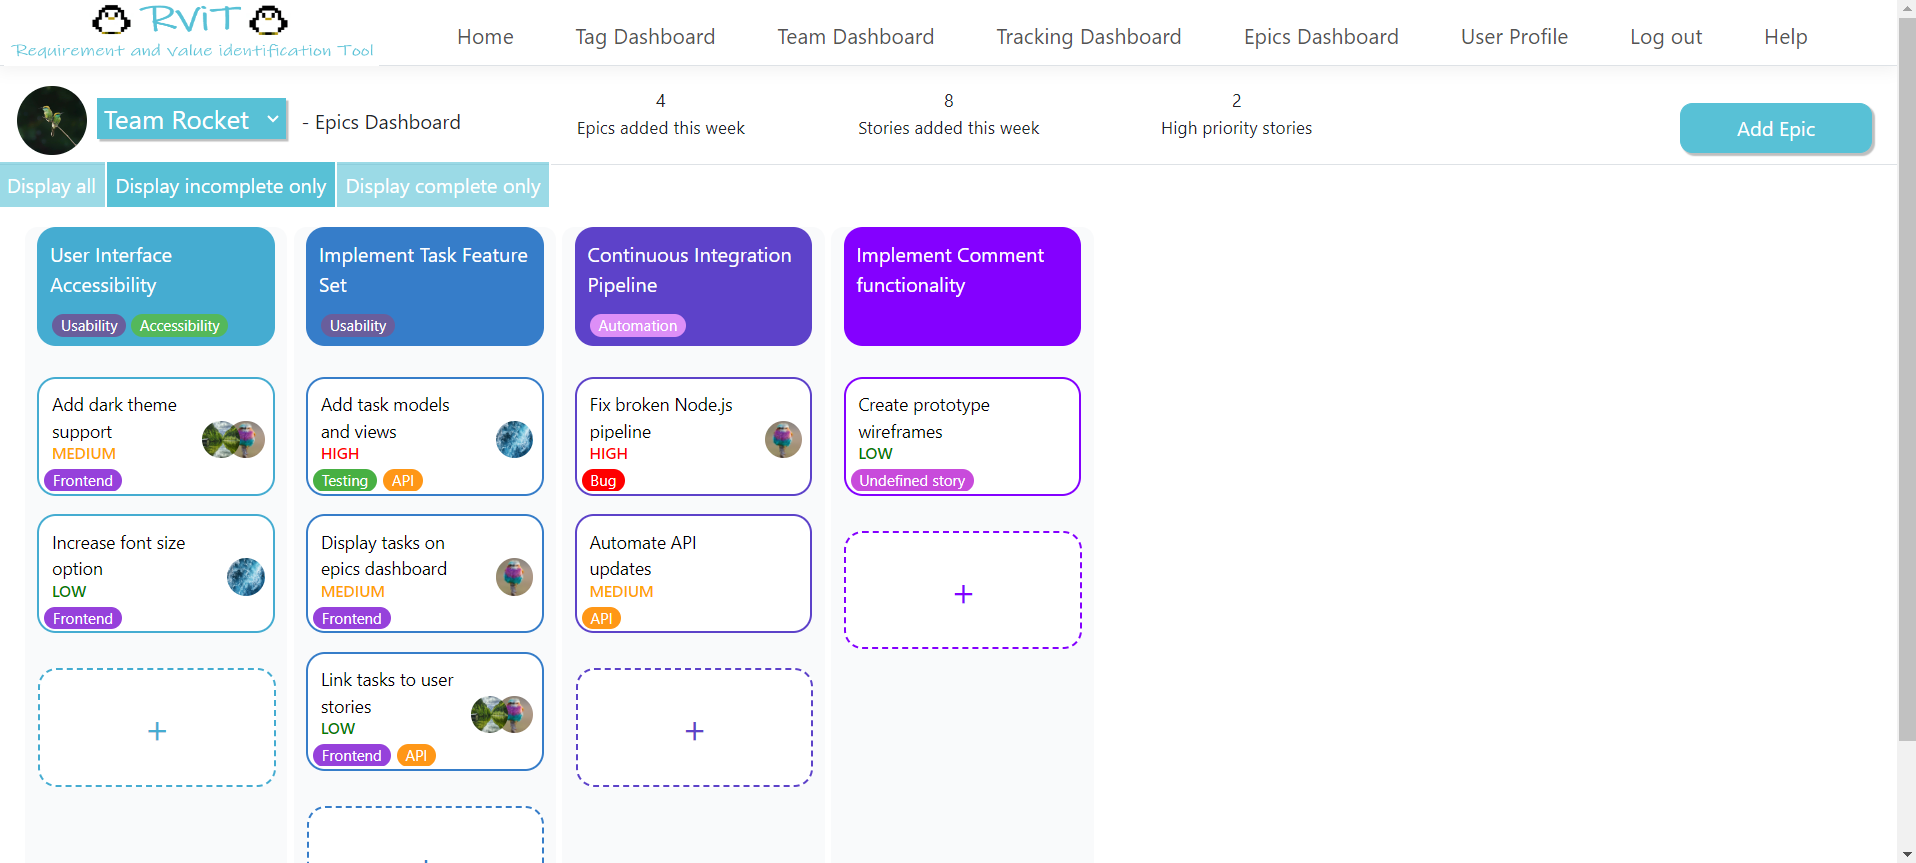
\includegraphics[scale=0.35]{dissertation/images/EpicsDashboard.png}
\caption{Epics Dashboard with example epics and user stories added}
\label{fig:epics dashboard} 
\end{center}
\end{figure}

\subsection{Epic and User Story Detail Modals}
As outlined in the requirements \textbf{MH.6} and \textbf{MH.7}, authorised team lead and team member users should be able to view and edit epic and user story details. It was decided that navigational overhead should be as little as possible. Therefore, instead of opening the editable details view on another page, a modal should be added on the Epics Dashboard. When examining other market-leading agile project management tools, it was found this also follows industry convention. 

The epic and user story detail views can be opened through their respective components on the Epics Dashboard. These views include all the relevant information about the element, satisfying \textbf{MH.6}. Both of the detail views are also editable, fulfilling requirement \textbf{MH.7}. Later in the project "Created by" and "Last edited by" logging information was also added to the details view, meeting \textbf{CH.2}. Both detail views allow an authorised user to delete the epic/user story in editing mode, fulfilling requirement \textbf{SH.5}. The epic detail editing view also contains a button which allows the user to manually mark it as completed. The finalised epic and user story detail modals can be seen in \textbf{Fig, \ref{fig:detail modals}}. Enlarged versions of these figures can be seen in \textbf{Appendix \ref{app: epics and us details}}.


\begin{figure}[h!]
\centering
\begin{subfigure}{.5\textwidth}
\centering
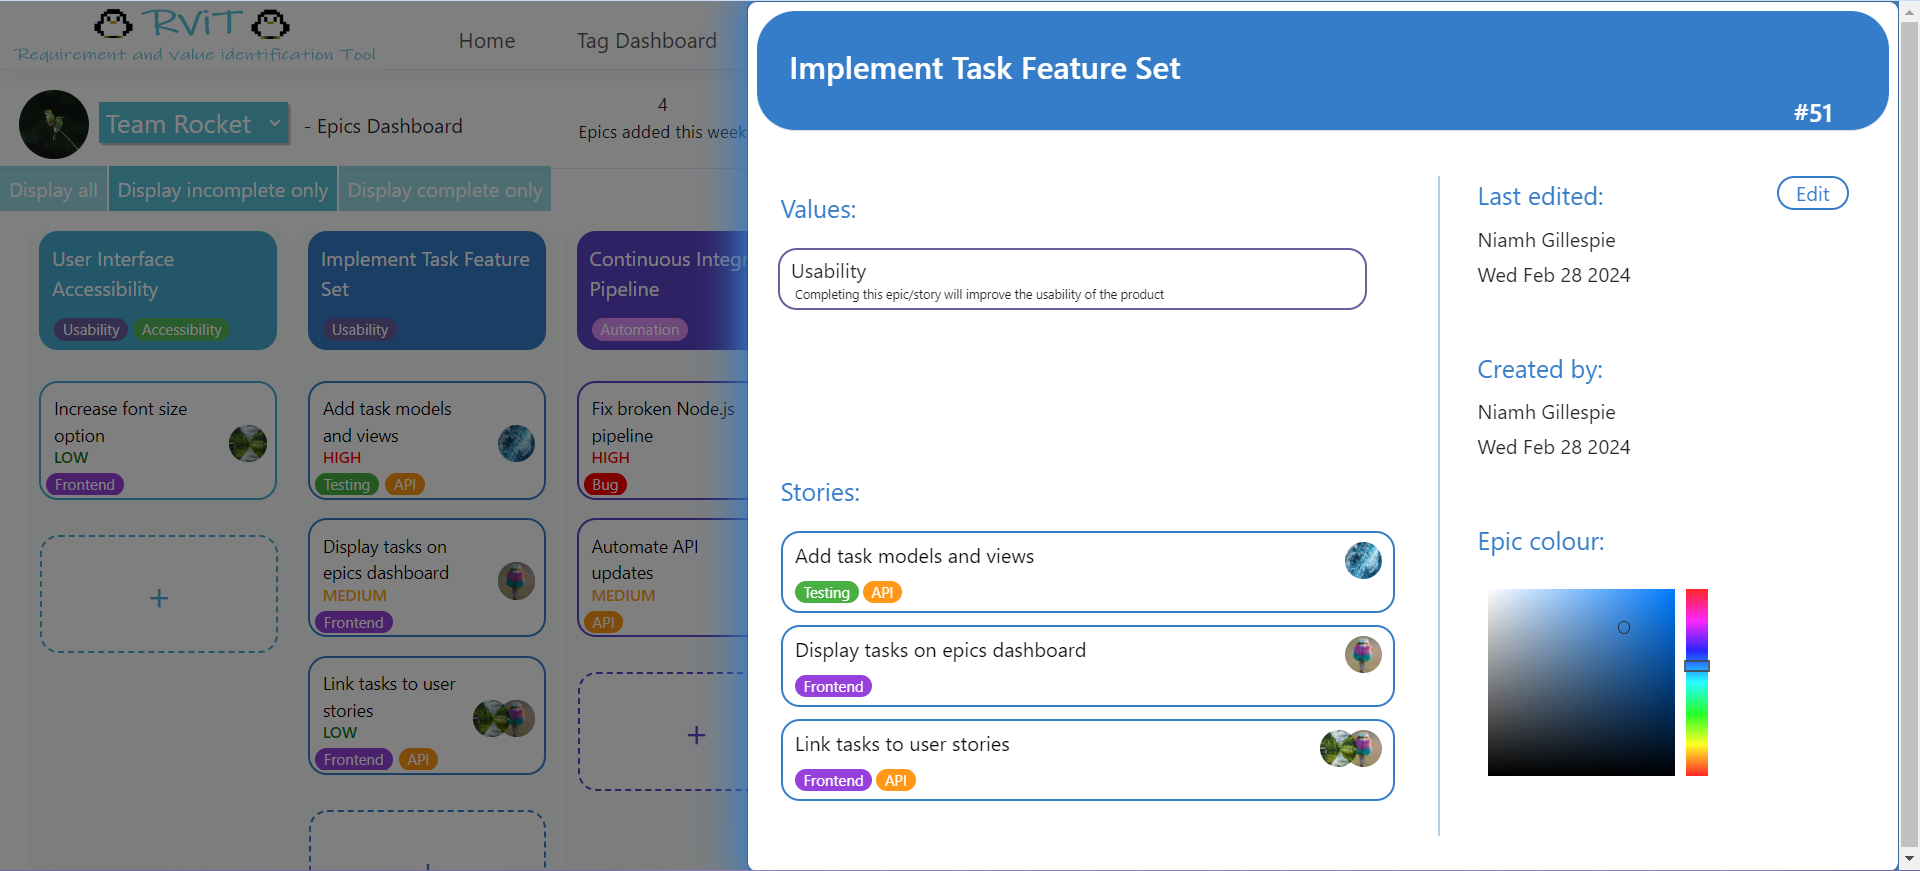
\includegraphics[scale=0.17]{dissertation/images/EpicDetails.png}
\caption{Epic details modal}
\end{subfigure}%
\begin{subfigure}{.5\textwidth}
\centering
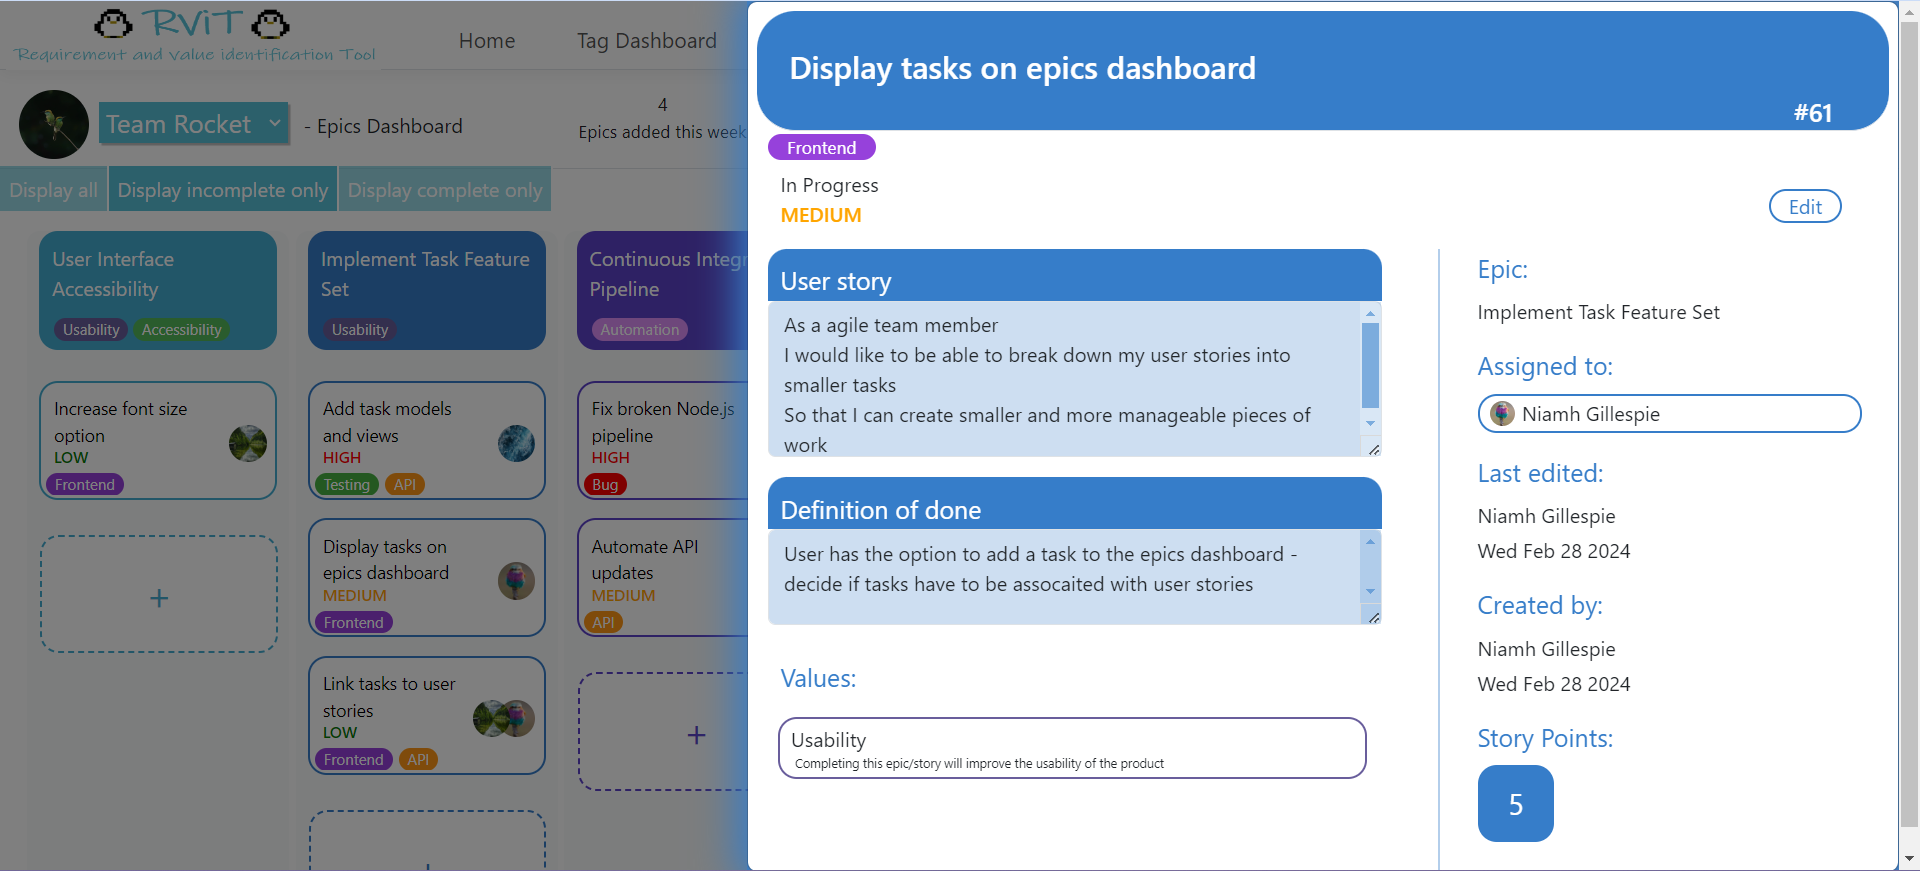
\includegraphics[scale=0.17]{dissertation/images/StoryDetails.png}
\caption{Story details modal}
\end{subfigure}

\caption{Epic and user story detail modals}
\label{fig:detail modals}
\end{figure}

\subsection{Tags Dashboard}
The Tags Dashboard is responsible for fulfilling requirement \textbf{MH.8}. Here, an authorised team lead or team member user can add both tags and values for their team to use. As mentioned in \textbf{Section 4.2.2}, these elements are fully colour customisable with colour-vs-text feedback on both creation and when editing the element. Both tags and values have an optional description field which allow users to express the purpose of the element. 

Both epics and user stories can add business value to a project, so authorised users are able to add value tags to both components. To increase the visibility of these business values, the epic components on the Epics Dashboard will display the value title, with the description displayed when a user hovers over the element, as seen in \textbf{Fig. \ref{fig:epics dashboard}} and \textbf{Fig. \ref{fig:tracking dashboard}}. While an element's assigned values are viewable on both the epic and user story detail views, to avoid a cluttered user interface it was decided against displaying values on the user story components as well. Stakeholders and project managers are also more likely to focus on the business value an epic brings, rather than the more fine-grained stories that belong to it. 

As tags will be used to categorise a user story into the areas of development a task will require, these can only be added to user stories. As seen in \textbf{Fig. \ref{fig:epics dashboard}} and \textbf{Fig. \ref{fig:tracking dashboard}}, these tags are displayed on the user stories components to allow developers to gain an understanding of story requirements without having to read through the user story and the definition of done in the details view. 

In order to allow for a user to add both tags and values seamlessly, the Tags Dashboard was created. To reduce the cluttering of the interface, an authorised user can toggle between viewing tags and values instead of viewing both at once, as seen in \textbf{Fig. \ref{fig:tag dashboard}}. Enlarged versions of these figures can be seen in \textbf{Appendix \ref{app: large tag and value views}}.


\begin{figure}[h!]
\centering
\begin{subfigure}{.5\textwidth}
\centering
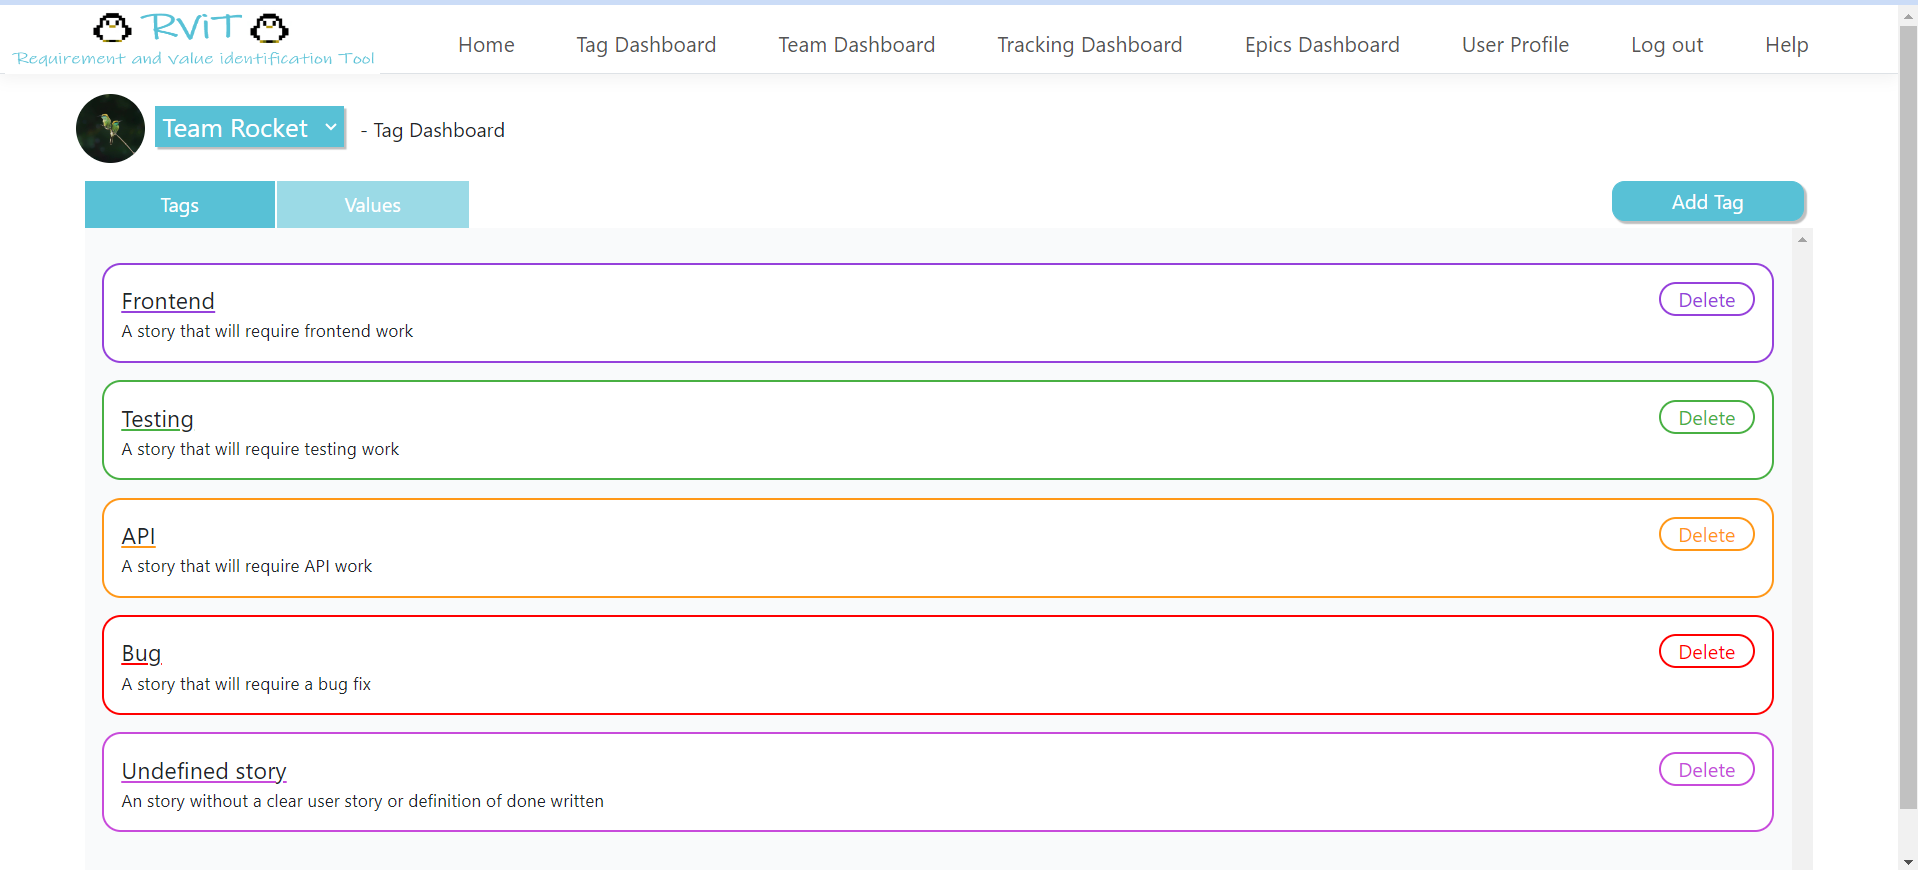
\includegraphics[scale=0.17]{dissertation/images/TagDashboardOne.png}
\caption{Tag dashboard - tag overview}
\end{subfigure}%
\begin{subfigure}{.5\textwidth}
\centering
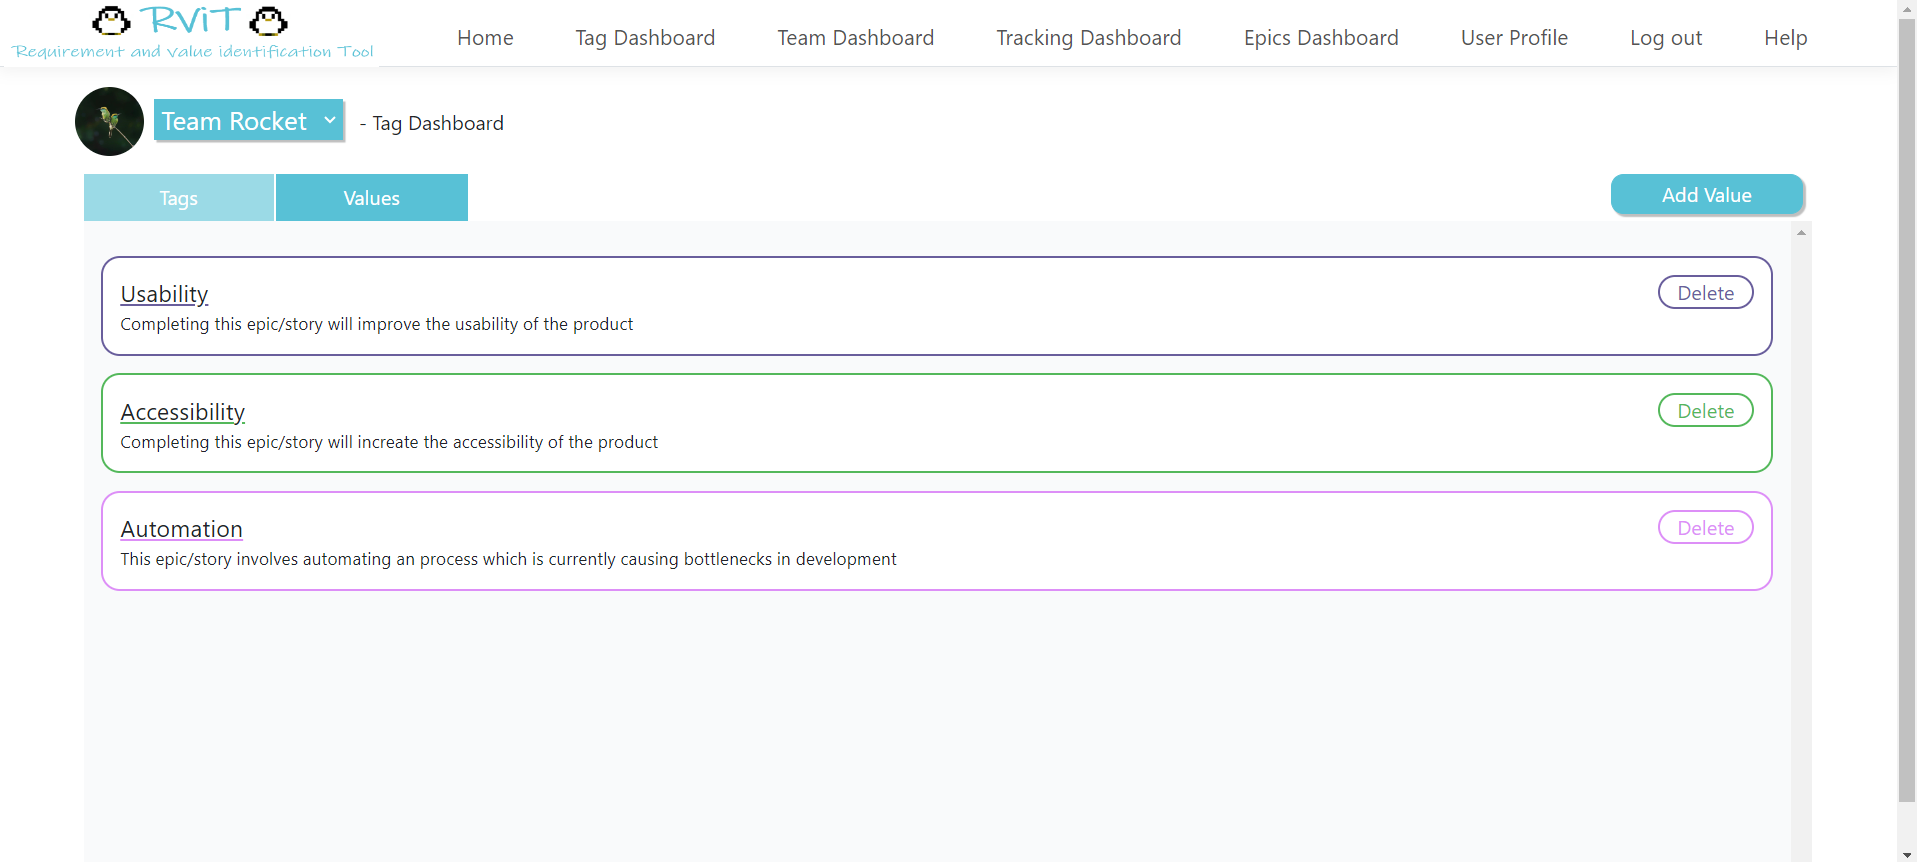
\includegraphics[scale=0.17]{dissertation/images/TagDashboardTwo.png}
\caption{Tag dashboard - values overview}
\end{subfigure}

\caption{Tag dashboard with example tags and values}
\label{fig:tag dashboard}
\end{figure}

\subsection{Tracking Dashboard}
The Tracking Dashboard allows a team to define a customised kanban board. Team member and team lead users can add as many tracking columns as they wish to fit their team's chosen workflow. This fulfils requirement \textbf{SH.3}. Each column has an optional WIP limit that can be set. To allow for maximum user flexibility, instead of prohibiting a user from moving a story into a column if it is over the WIP limit, the column's border is changed from blue to red. This way users are still alerted that the WIP limit has been reached, while still allowing for use cases where the WIP limit should be overruled.

Authorised users can add multiple user stories to a tracking column at once and move these stories between defined columns using drag and drop, satisfying requirement \textbf{MH.9}.

Users can also choose to automatically mark stories as completed once they have entered a specified column, as seen in \textbf{Fig. \ref{fig:tracking dashboard}}, fulfilling \textbf{CH.1}. To visually distinguish these from non-completed stories, a completed banner is added to the story.

Similarly to the Epics Dashboard, the user story components can be clicked to bring up their details view. This was overlooked in the original design process, but when building and manually testing the Tracking Dashboard, it became apparent that this view would be heavily used in stand-up meetings where users are likely to want to view and edit story details. For instance, team members who have just finished work would likely be assigned new work from a backlog column. 

Time-based filters were also added to the Tracking Dashboard when considering the user experience. These filters allow users to view the stories which have been edited in the last 24, 48 and 72 hours, reducing the number of stories displayed on the dashboard and allowing teams to focus on the current workflow. This is also a feature designed with stand-up meetings in mind, as it could help teams identify story blockers or reduce the team's scope of attention to only those stories who have moved column in the last 24 hours.

\begin{figure}[h!]
\begin{center}
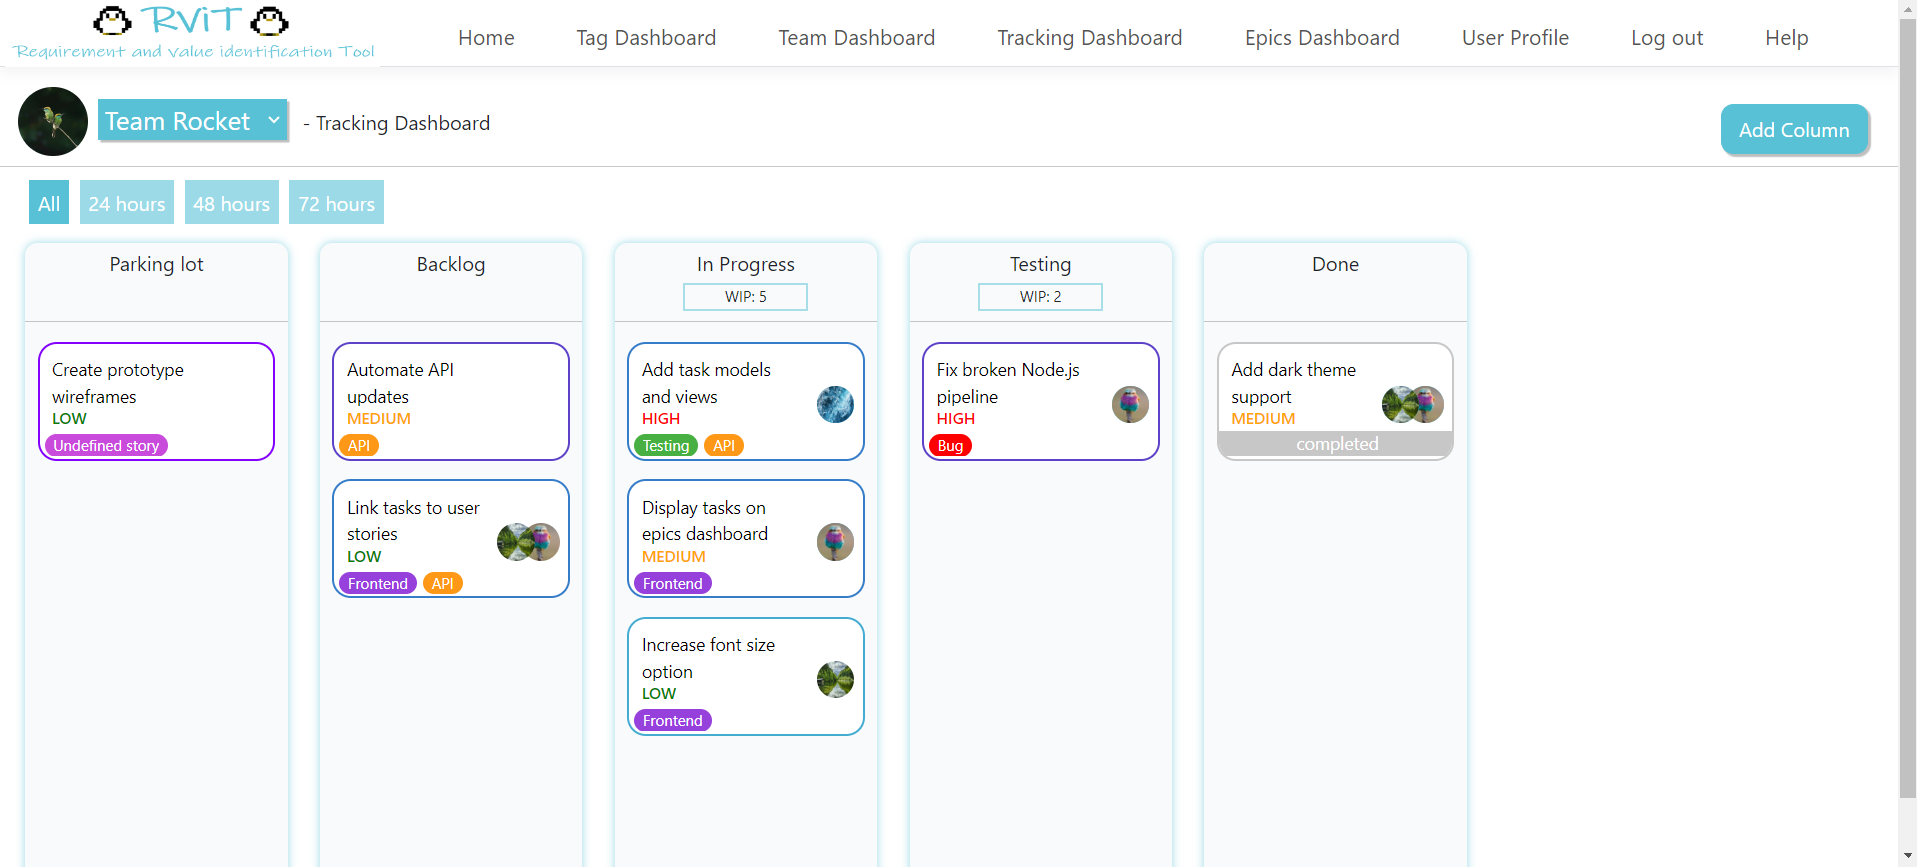
\includegraphics[scale=0.35]{dissertation/images/TrackingDashboard.png}
\caption{Tracking Dashboard with example user stories added}
\label{fig:tracking dashboard} 
\end{center}
\end{figure}


\subsection{Admin Workflow}
An admin user is able to add teams and users to their organisation via the 'Add Team' and 'Add User' pages. These pages fulfil requirements \textbf{MH.12} and \textbf{MH.13}.

The View Teams page allows an admin user to view a team's overview page, as well as edit and delete teams, satisfying requirements \textbf{MH.14} and \textbf{MH.15}. This page also features on-type search functionality to allow admin users of larger organisations to find teams effectively.

Similarly, the View Users page allows an admin user to view a user's profile, edit a user's details and delete a user, again satisfying requirements \textbf{MH.14} and \textbf{MH.15}. On this page, admin users can filter by user type as well as use on-type search functionality to effectively find users.

These pages can be found in \textbf{Appendix \ref{app: admin workflow}}

\subsection{User authentication}
As RViT was primarily designed with small to medium organisations in mind, the sign-up process is greatly simplified. When completing the initial sign-up process a user can enter the name of their organisation and create an admin account. As explained in \textbf{Section 4.2.6}, an administration user can then create other admin users, as well as team leads and team members. 

Both the login and sign-up pages can be viewed in \textbf{Appendix \ref{app: user authentication workflow}}

\section{Tools and Technologies}
Appropriate tools and technologies for development were identified at the beginning of the project. The choice of these were not restricted by any of the functional or non-functional requirements. As the project was anticipated to involve implementing vast amounts of functionality, care was taken to ensure the author had experience with the majority of the tooling used. 

\subsection{Frontend}
Creating an aesthetically pleasing and easily usable application was core to creating a product that could compete with the numerous established agile project management tools currently on the market. With the high levels of user interaction needed on the frontend, using a JavaScript framework was an obvious choice. 

A key reason that React JS was chosen was because of its support for reusable components. Not only does this reduce the reused code in a project, making the code base more readable, but individual components can be updated without the need to reload the full we page. This was vital when creating RViT, as there are many separate components that can be edited and updated without a need to reload the full page. 

React also has an extremely strong developer community, with hundreds of ready-to-use component packages available. This project makes use of some of these packages such as React Bootstrap, PrimeReact's colour picker and react-beautiful-dnd which was used to implement the drag and drop functionality on the Tracking and Epics Dashboards.

Front end styling was done through a combination of bootstrap and external CSS. The only exception to this being the inline CSS that was used for the majority of the colour functionality in the frontend.

\subsection{API}
Django was chosen to build the application layer due to its built-in REST API support. The Django REST Framework allows developers to create an easily accessible, web-browsable, API. This support means that endpoints can be tested from a web browser, simplifying the manual testing and debugging process. This feature was extremely helpful over the course of development as it greatly simplified the error finding and debugging process. 

The Django REST Framework also handles data serialization and deserialization, allowing Python data types and objects to be parsed into JSON and sent to the presentation layer and vice versa. This greatly simplified the passing of data to and from the API as little data formatting had to be carried out on either the application or presentation tiers. 


\subsection{Database}
SQLite was chosen as a database primarily due to its lightweight nature and out-of-the-box support for Django. SQLite's atomic transactions means that database updates are either carried out fully or not at all, even during system outages. Therefore, data will not be corrupted even in the case of a system outage partially through a write sequence.

Hosting the project was also a concern due to the sizable nature of the code base, so SQLite was an ideal choice as the majority of other databases would take up much more disk space than is normally provided on free hosting tiers. Due to SQLite's lightweight nature, it also typically performs better than other databases, an aspect essential to this project, due to the numerous read/write operations that will occur during typical use.

While SQLite works well for small to medium applications, if future larger-scale development was pursued, a database more suited to large applications with high levels of concurrency support could be investigated.

The finalised database schema can be seen in \textbf{Appendix \ref{app: database}}
\end{document}